\setcounter{section}{0}

\begin{enumerate}[label=\bfseries Câu \arabic*:]
		\item \mkstar{2}
	
	{
		
		Một lực có độ lớn $\SI{6}{N}$ tác dụng lên vật có khối lượng $\SI{0,5}{kg}$ đang đứng yên. Bỏ qua ma sát và các lực cản. Gia tốc của vật bằng bao nhiêu?
		
	}
	
	\hideall{
		
		Gia tốc của vật là:
		
		$$a = \dfrac{F}{m} = \SI{12}{m/s}^2.$$
	}
	\item \mkstar{3}
	
	{
		Xét một ô tô có khối lượng $\SI{900}{kg}$ đang đi với vận tốc $\SI{20}{m/s}$ thì người lái xe nhìn thấy đèn giao thông chuyển màu đỏ ở phía trước. Để xe giảm tốc độ và dừng lại sau $\SI{10}{s}$ thì lực hãm khi phanh ô tô phải là bao nhiêu?
	}
	
	\hideall{
		
	Gia tốc của ô tô cần có để giảm tốc và dừng lại là:
	
	$$a = \dfrac{\Delta v}{\Delta t} = -\SI{2}{m/s}^2.$$
	
	Lực hãm phanh được xác đinh:
	
	$$F = ma = - \text{1,8} \cdot 10^3\ \text{N}.$$
	
	Như vậy, độ lớn lực hãm khi phanh là $\text{1,8}\cdot 10^3\ \text{N}$ để xe giảm tốc và dừng lại sau $\SI{10}{s}$ từ vận tốc $\SI{20}{m/s}$. Dấu "=" thể hiện lực ngược chiều chuyển động, gây ra gia tốc ngược hướng vận tốc.
	}
	
	\item \mkstar{3}
	
	{
		
		Mẫu xe điện có thời gian tăng tốc nhanh nhất được thử nghiệm đã tăng tốc từ $\SI{0}{km/h}$ đến $\SI{97}{km/h}$ trong 1,98 giây. Hãy tính gia tốc của xe và lực để tạo ra gia tốc đó. Coi xe chuyển động biến đổi đều và khối lượng của mẫu xe này là 2 tấn.
	}
	
	\hideall{
		
		Đổi $\SI{97}{km/h} = \SI{26,94}{m/s}.$
		
		Ta có:
		
		$$a = \dfrac{v - v_0}{t} = \SI{13,61}{m/s}^2.$$
		
		Mà: 
		
		$$F = ma = \SI{27220}{kg\cdot m/s}^2.$$
		
	}
	\item \mkstar{3}
	
	{
		
		Thông số mẫu xe ô tô được cung cấp như bảng dưới đây. Tính lực tác dụng để mẫu xe trên chở đủ tải trọng và tăng tốc từ trạng thái nghỉ đến tốc độ tối ưu trong 2 giây.
		
		\begin{center}
			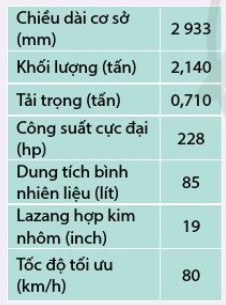
\includegraphics[scale=1]{../figs/VN10-2022-PH-TP016-1.jpg}
		\end{center}
		
	}
	
	\hideall{
		
		Để xe trên chở đủ tải trọng và tăng tốc từ trạng thái nghỉ đến tốc độ tối ưu trên 2 giây thì gia tốc của xe là:
		
		$$a = \dfrac{v - v_0}{t} = \SI{11,11}{m/s}^2.$$
		
		Lực tác dụng là
		
		$$F = ma= \SI{31663,5}{N}.$$
	}
	\item \mkstar{3}
	
	{
		
		Một người có khối lượng $\SI{60}{kg}$ đi trên xe đạp có khối lượng $\SI{20}{kg}$. Khi xuất phát, hợp lực tác dụng lên xe đạp là $\SI{200}{N}$. Giả sử hợp lực tác dụng lên xe đạp không đổi, hãy tính vận tốc của xe đạp sau $\SI{5}{s}$.
	}
	
	\hideall{
		
		Xe đạp đi với gia tốc là:
		
		$$a=\dfrac{F}{m}= \SI{2,5}{m/s}^2.$$
		
		Vận tốc của xe đạp sau $\SI{5,00}{s}$ là:
		
		$$v=v_0+at = \SI{12,5}{m/s}.$$
		
	}

		\item \mkstar{3}
	
	{
		
		Một ô tô có khối lượng 1 tấn đang chuyển động với $v = \SI{54}{km/h}$ thì tắt máy, hãm phanh, chuyển động chậm dần đều. Biết độ lớn lực hãm $\SI{3000}{N}$. Xác định quãng đường xe đi được cho đến khi dừng lại.
	}
	
	\hideall{
		
		Do đây là lực hãm nên sẽ mang giá trị âm.
		
		Gia tốc của vật:
		
		$$a = \dfrac{-F}{m} = -\SI{3}{m/s}^2.$$
		
		Khi xe dừng ta có $v=0$ ta có:
		
		$$s = \dfrac{v^2 - v_0^2}{2a} = \SI{37,5}{m}.$$
	}
	
	\item \mkstar{3}
	
	{
		
		Lực không đổi tác dụng vào vật $m_1$ gây gia tốc $\SI{4}{m/s}^2$; tác dụng vào vật $m_2$ gây ra gia tốc $\SI{5}{m/s}^2.$ Tính gia tốc của vật có khối lượng $m_1 + m_2$ chịu tác dụng của lực trên.
	}
	
	\hideall{
		
		Ta có:
		
		$$a = \dfrac{F}{m_1 + m_2} = \dfrac{F}{\dfrac{F}{a_1}+ \dfrac{F}{a_2}} = \dfrac{1}{\dfrac{1}{a_1}+ \dfrac{1}{a_2}} = \SI{0,22}{m/s}^2.$$
		
	}
	\item \mkstar{3}
	
	{
		Một vật có khối lượng $\SI{50}{kg}$, bắt đầu chuyển động nhanh dần đều và sau khi đi được $\SI{1}{m}$ thì có vận tốc $\SI{0,5}{m/s}$. Tính lực tác dụng vào vật.
	}
	
	\hideall{
		
		Chọn chiều dương là chiều chuyển động ta có:
		
		$$v^2 - v^2_0 = 2as \Rightarrow a = \SI{0,125}{m/s}^2.$$
		
		Lực tác dụng lên vật
		
		$$F = ma = \SI{6,25}{N}.$$
	}
	\item \mkstar{3}
	
	{
		Một quả bóng có khối lượng $\SI{500}{g}$ đang nằm trên sân cỏ. Sau khi bị đá nó có vận tốc $v = \SI{2}{m/s}$. Tính lực đá của cầu thủ. Biết khoảng thời gian va chạm là $t = \SI{0,02}{s}$.
	}
	
	\hideall{
		
		Chọn chiều dương là chiều chuyển động:
		
		$$v = v_0 + at \Rightarrow a = \SI{100}{m/s}^2 (v_0 = 0).$$
		
		Lực đá của cầu thủ
		
		$$F = ma = \SI{50}{N}.$$
		
		
		
	}
	\item \mkstar{3}
	
	{
		
		Lần lượt tác dụng lực có độ lớn $F_1$ và $F_2$ lên một vật có khối lượng $m$, vật thu được gia tốc có độ lớn lần lượt là $a_1$ và $a_2$. Biết $3F_1 = 5F_2$. Bỏ qua mọi ma sát. Tỉ số $\dfrac{a_1}{a_2}$ là bao nhiêu?
	}
	
	\hideall{
		
		Ta có: 
		
		$$3F_1 = 5F_2 \Rightarrow \dfrac{F_1}{F_2} = \dfrac{5}{3}.$$
		
		Suy ra:
		
		$$ \dfrac{F_1}{F_2} = \dfrac{ma_1}{ma_2} = \dfrac{a_1}{a_2} = \dfrac{5}{3}.$$
		
	}
	
\end{enumerate}